\documentclass[12pt,a4paper]{article}

% Packages
\usepackage{geometry}
\geometry{margin=1in}
\usepackage{fancyhdr}
\usepackage{titlesec}
\usepackage{listings}
\usepackage{xcolor}
\usepackage{graphicx} 

% Header & Footer
\pagestyle{fancy}
\fancyhf{}
\rhead{C++ - Assignment 2}
\lhead{Kamithkar Vinod}
\cfoot{\thepage}

% Title formatting
\titleformat{\section}{\large\bfseries}{Problem \thesection:}{0.5em}{}
\titleformat{\subsection}[runin]{\bfseries}{Code:}{0.5em}{}[---]
\titleformat{\subsubsection}[runin]{\bfseries}{Output:}{0.5em}{}[---]

% Code style
\lstset{
    language=cpp,
    basicstyle=\ttfamily\small,
    keywordstyle=\color{blue}\bfseries,
    commentstyle=\color{gray}\itshape,
    stringstyle=\color{red},
    showstringspaces=false,
    numbers=left,
    numberstyle=\tiny\color{gray},
    frame=single,
    breaklines=true
}

% Document Start
\begin{document}

% Title Page
\begin{center}
    \LARGE \textbf{Assignment - 2} \\[0.5cm]
    \Large \textbf{C++} \\[1cm]

    \begin{tabular}{rl}
        \textbf{Name:} & Kamithkar Vinod \\
        \textbf{Course:} & PG DAC AUGUST 2025 \\
        \textbf{PRN:} & 250850320040 \\
        \textbf{Form No:} & 250500480 \\
        \textbf{Date:} & 08-10-2025 \\
    \end{tabular}
\end{center}

\vspace{1cm}
\hrule
\vspace{0.5cm}

% Problems
% 1
\section{Basic Pointer }
\textbf{Task:} Write a program in C++ to declare an integer variable, store its address in a pointer, and display both the value of the variable and its address using the pointer.


\subsection{}
\begin{lstlisting}
#include <iostream>
using namespace std;

int main() {
    int num = 10;
    int *ptr = &num;

    cout << "Value of num: " << num << endl;
    cout << "Address of num using pointer: " << ptr << endl;
    cout << "Value accessed through pointer: " << *ptr << endl;
    return 0;
}

\end{lstlisting}

\subsubsection{1}
\begin{center}
    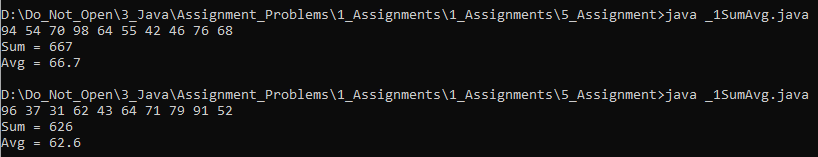
\includegraphics[width=0.8\textwidth]{1.png}
\end{center}


% 2

\section{Pointer Arithmetic}
\textbf{Task:} Write a program in C++ to create an array of 5 integers. Use a pointer to traverse the array and print all elements using pointer arithmetic. 
\subsection{}
\begin{lstlisting}
#include <iostream>
using namespace std;

int main() {
    int arr[5] = {10, 20, 30, 40, 50};
    int *ptr = arr;

    cout << "Array elements using pointer arithmetic:\n";
    for (int i = 0; i < 5; i++) {
        cout << *(ptr + i) << " ";
    }
    return 0;
}

\end{lstlisting}

\subsubsection{}
\begin{center}
    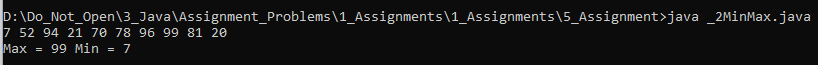
\includegraphics[width=0.8\textwidth]{2.png}
\end{center}

% 3

\section{Call by Reference (using pointer)}
\textbf{Task:} Write a program in C++ to swap two numbers using pointers. 

\subsection{}
\begin{lstlisting}
#include <iostream>
using namespace std;

void swapNumbers(int *a, int *b) {
    int temp = *a;
    *a = *b;
    *b = temp;
}

int main() {
    int x = 5, y = 10;
    cout << "Before Swap: x = " << x << ", y = " << y << endl;

    swapNumbers(&x, &y);

    cout << "After Swap: x = " << x << ", y = " << y << endl;
    return 0;
}
\end{lstlisting}

\subsubsection{}
\begin{center}
    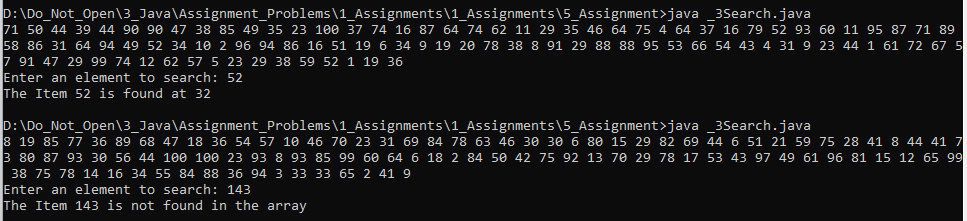
\includegraphics[width=0.8\textwidth]{3.png}
\end{center}

% 4

\section{Dynamic Memory Allocation}
\textbf{Task:} Write a program in C++ to dynamically allocate memory for an array of 5 integers using a pointer, take input from the user, and display the array elements. 

\subsection{}
\begin{lstlisting}
#include <iostream>
using namespace std;

int main() {
    int *arr = new int[5];

    cout << "Enter 5 integers: ";
    for (int i = 0; i < 5; i++) {
        cin >> arr[i];
    }

    cout << "Array elements: ";
    for (int i = 0; i < 5; i++) {
        cout << arr[i] << " ";
    }

    delete[] arr;
    return 0;
}

\end{lstlisting}

\subsubsection{}
\begin{center}
    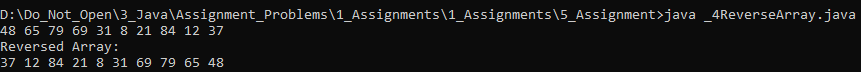
\includegraphics[width=0.8\textwidth]{4.png}
\end{center}

% 5

\section{Function with Pointer }
\textbf{Task:} Write a program in C++ to pass a pointer to a function that updates the value of a variable. 

\subsection{}
\begin{lstlisting}
#include <iostream>
using namespace std;

void updateValue(int *p) {
    *p = *p + 10;
}

int main() {
    int num = 5;
    cout << "Before update: " << num << endl;

    updateValue(&num);

    cout << "After update: " << num << endl;
    return 0;
}

\end{lstlisting}

\subsubsection{}
\begin{center}
    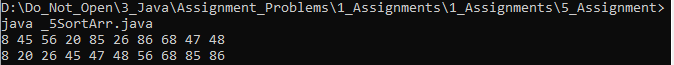
\includegraphics[width=0.8\textwidth]{5.png}
\end{center}

% 6

\section{String with Pointers }
\textbf{Task:} Write a program in C++ to count the length of a string using a character pointer (without using built-in functions like strlen).

\subsection{}
\begin{lstlisting}
#include <iostream>
using namespace std;

int main() {
    char str[100];
    cout << "Enter a string: ";
    cin.getline(str, 100);

    char *ptr = str;
    int length = 0;

    while (*ptr != '\0') {
        length++;
        ptr++;
    }

    cout << "Length of string: " << length << endl;
    return 0;
}

\end{lstlisting}

\subsubsection{}
\begin{center}
    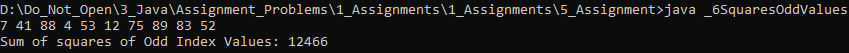
\includegraphics[width=0.8\textwidth]{6.png}
\end{center}

% 7

\section{Dynamic Integer}
\textbf{Task:} Write a program in C++ to dynamically allocate memory for a single integer using new, assign a value, display it, and then free the memory using delete. 

\subsection{}
\begin{lstlisting}
#include <iostream>
using namespace std;

int main() {
    int *ptr = new int;
    *ptr = 25;

    cout << "Value: " << *ptr << endl;

    delete ptr;
    return 0;
}

\end{lstlisting}

\subsubsection{}
\begin{center}
    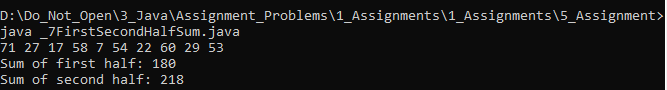
\includegraphics[width=0.8\textwidth]{7.png}
\end{center}

% 8

\section{Dynamic Array }
\textbf{Task:} Write a program in C++ to create an array of 5 integers using new, take input from the user, display the array elements, and then release the memory using delete[].

\subsection{}
\begin{lstlisting}
#include <iostream>
using namespace std;

int main() {
    int *arr = new int[5];

    cout << "Enter 5 integers: ";
    for (int i = 0; i < 5; i++) {
        cin >> arr[i];
    }

    cout << "Array elements: ";
    for (int i = 0; i < 5; i++) {
        cout << arr[i] << " ";
    }

    delete[] arr;
    return 0;
}

\end{lstlisting}

\subsubsection{}
\begin{center}
    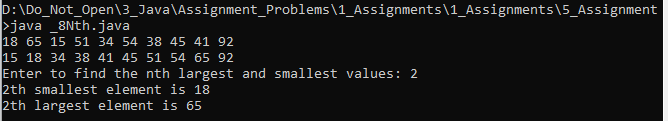
\includegraphics[width=0.8\textwidth]{8.png}
\end{center}

% 9

\section{Dynamic 2D Array }
\textbf{Task:} Write a program in C++ to create a 2D array (matrix) dynamically using new. Take input for rows and columns from the user, fill the matrix, display it, and free memory using delete[].

\subsection{}
\begin{lstlisting}
#include <iostream>
using namespace std;

int main() {
    int rows, cols;
    cout << "Enter rows and columns: ";
    cin >> rows >> cols;

    int **matrix = new int*[rows];
    for (int i = 0; i < rows; i++)
        matrix[i] = new int[cols];

    cout << "Enter matrix elements:\n";
    for (int i = 0; i < rows; i++)
        for (int j = 0; j < cols; j++)
            cin >> matrix[i][j];

    cout << "Matrix:\n";
    for (int i = 0; i < rows; i++) {
        for (int j = 0; j < cols; j++)
            cout << matrix[i][j] << " ";
        cout << endl;
    }

    for (int i = 0; i < rows; i++)
        delete[] matrix[i];
    delete[] matrix;

    return 0;
}

\end{lstlisting}

\subsubsection{}
\begin{center}
    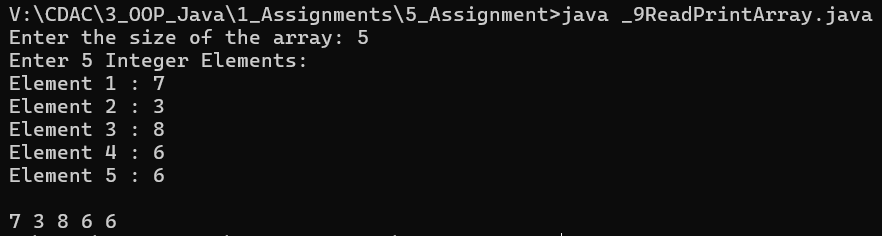
\includegraphics[width=0.8\textwidth]{9.png}
\end{center}

% 10

\section{Dynamic String }
\textbf{Task:} Write a program in C++ to dynamically allocate memory for a string using a character pointer and new. Take user input for the string, display it, and then free the memory. 

\subsection{}
\begin{lstlisting}
#include <iostream>
using namespace std;

int main() {
    int size;
    cout << "Enter the size of string: ";
    cin >> size;

    char *str = new char[size];
    cout << "Enter string: ";
    cin.ignore();
    cin.getline(str, size);

    cout << "You entered: " << str << endl;

    delete[] str;
    return 0;
}

\end{lstlisting}

\subsubsection{}
\begin{center}
    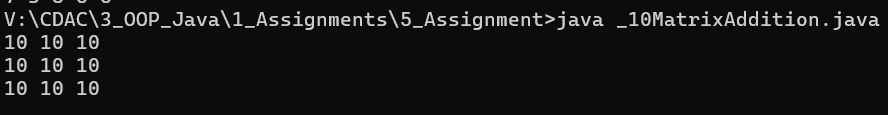
\includegraphics[width=0.8\textwidth]{10.png}
\end{center}

% 11

\section{Function Returning Dynamic Memory }
\textbf{Task:} Write a program in C++ with a function that returns a pointer to a dynamically allocated array. In main(), call the function, display the array, and free the memory.

\subsection{}
\begin{lstlisting}
#include <iostream>
using namespace std;

int* createArray(int n) {
    int *arr = new int[n];
    cout << "Enter " << n << " integers: ";
    for (int i = 0; i < n; i++)
        cin >> arr[i];
    return arr;
}

int main() {
    int n = 5;
    int *ptr = createArray(n);

    cout << "Array elements: ";
    for (int i = 0; i < n; i++)
        cout << ptr[i] << " ";

    delete[] ptr;
    return 0;
}

\end{lstlisting}

\subsubsection{}
\begin{center}
    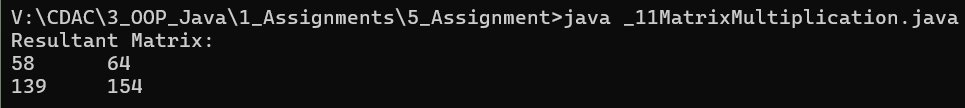
\includegraphics[width=0.8\textwidth]{11.png}
\end{center}

% 12

\section{Pointer Re-allocation (basic simulation) }
\textbf{Task:} Write a program in C++ to dynamically allocate an array of integers using new, fill it with values, then allocate a bigger array, copy the old values into it, add more elements, and release both old and new arrays properly.

\subsection{}
\begin{lstlisting}
#include <iostream>
using namespace std;

int main() {
    int n = 3;
    int *arr = new int[n];

    cout << "Enter 3 integers: ";
    for (int i = 0; i < n; i++)
        cin >> arr[i];

    int newSize = 5;
    int *newArr = new int[newSize];

    for (int i = 0; i < n; i++)
        newArr[i] = arr[i];

    cout << "Enter 2 more integers: ";
    for (int i = n; i < newSize; i++)
        cin >> newArr[i];

    cout << "New array: ";
    for (int i = 0; i < newSize; i++)
        cout << newArr[i] << " ";

    delete[] arr;
    delete[] newArr;
    return 0;
}

\end{lstlisting}

\subsubsection{}
\begin{center}
    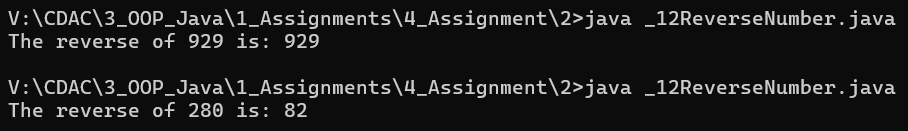
\includegraphics[width=0.8\textwidth]{12.png}
\end{center}

\end{document}



